\documentclass[12pt]{article}

\input preamble

\title{Principles of Parallel Architecture\\
Amdahl’s law and speed up}
\author{Xitong Liu \\
xliu@ece.udel.edu}

\begin{document}

\maketitle

\section{Serial Matrix Multiplication}
\begin{enumerate}

\item Serial Matrix Multiplication
\begin{description}
\item[Q:] 
\item[A:] 
\end{description}

\end{enumerate}
\end{document}

\begin{comment}
\begin{figure}[h!]
	\begin{center}
		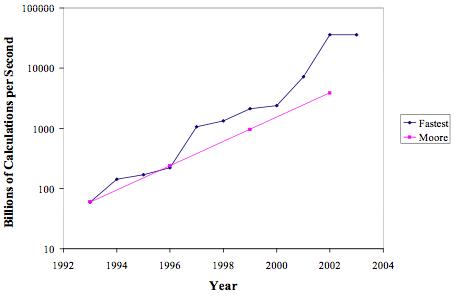
\includegraphics[width=0.7\textwidth, angle=0]{fatest.png}
		\caption{\label{fig:fatest}Fatest SuperComputer in the world}
	\end{center}
\end{figure}
\end{comment}